\documentclass[11pt]{article}

\usepackage{amsmath}
\usepackage{amssymb}

\usepackage{graphicx}
\usepackage{tikz}

\usepackage{ytableau}

\title{Planar graphs, UMTYMP Adv.~Topics, Fall 2020}
\date{}


\begin{document}


\maketitle

\thispagestyle{empty}

\vspace{-0.6in}

\begin{enumerate}
\item The \emph{wheel graph} $W_n$ on $n$ vertices is obtained from the cycle graph $C_{n-1}$ on $(n-1)$ vertices by adding a new vertex adjacent to every other vertex; for instance $W_6$ looks like:
\[  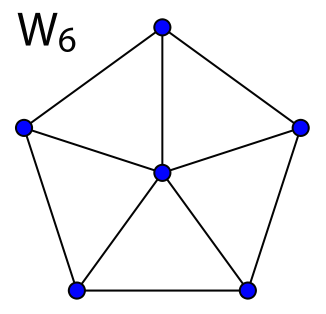
\includegraphics[width=0.9in]{wheel_graph.png} \]
Show that $W_n$ is always self-dual.
\item Show that the planar graphs corresponding to the icosahedron and dodecahedron are dual:
\[ 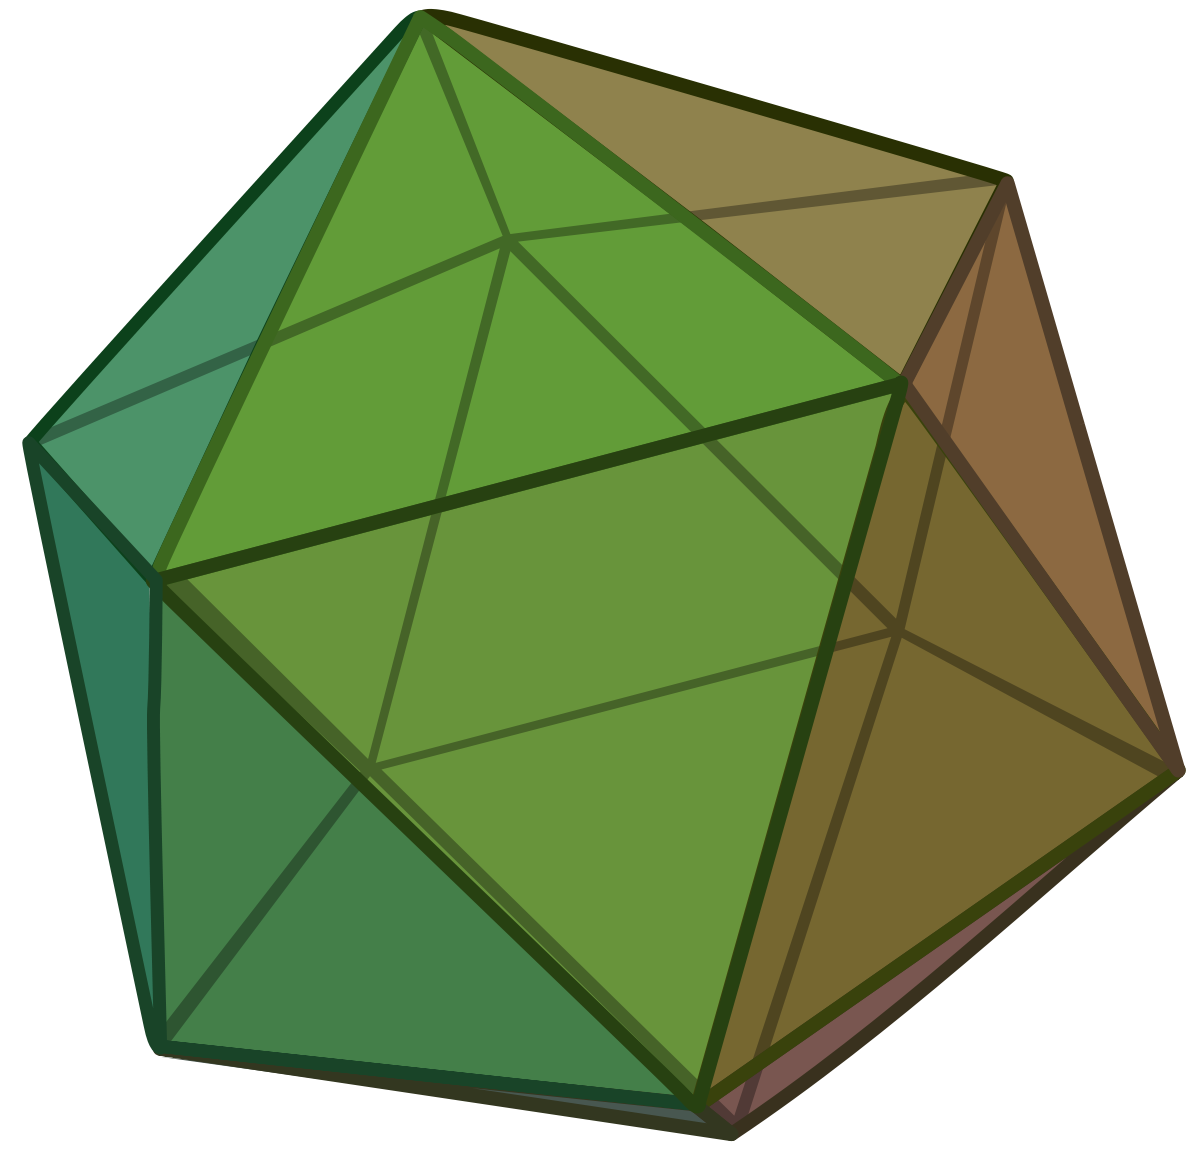
\includegraphics[width=0.9in]{icosahedron.png} \qquad \qquad \qquad 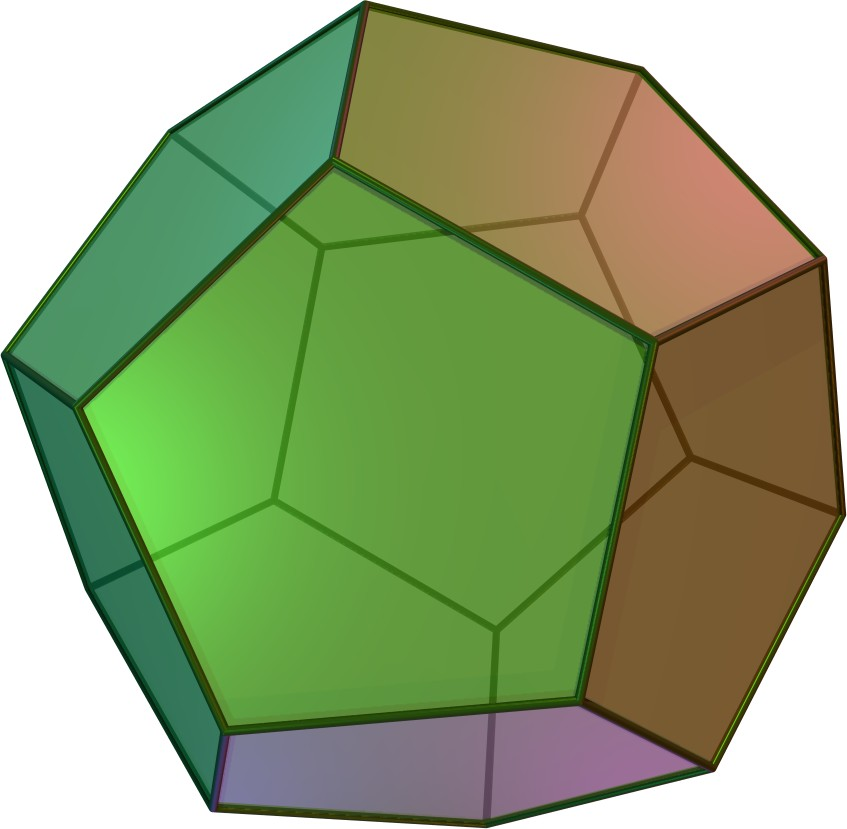
\includegraphics[width=0.9in]{dodecahedron_solid.png} \]
\item Explain why a planar graph $G$ and its dual $G^*$ have the same number of spanning trees.
\item Recall that the Petersen graph is
\[ 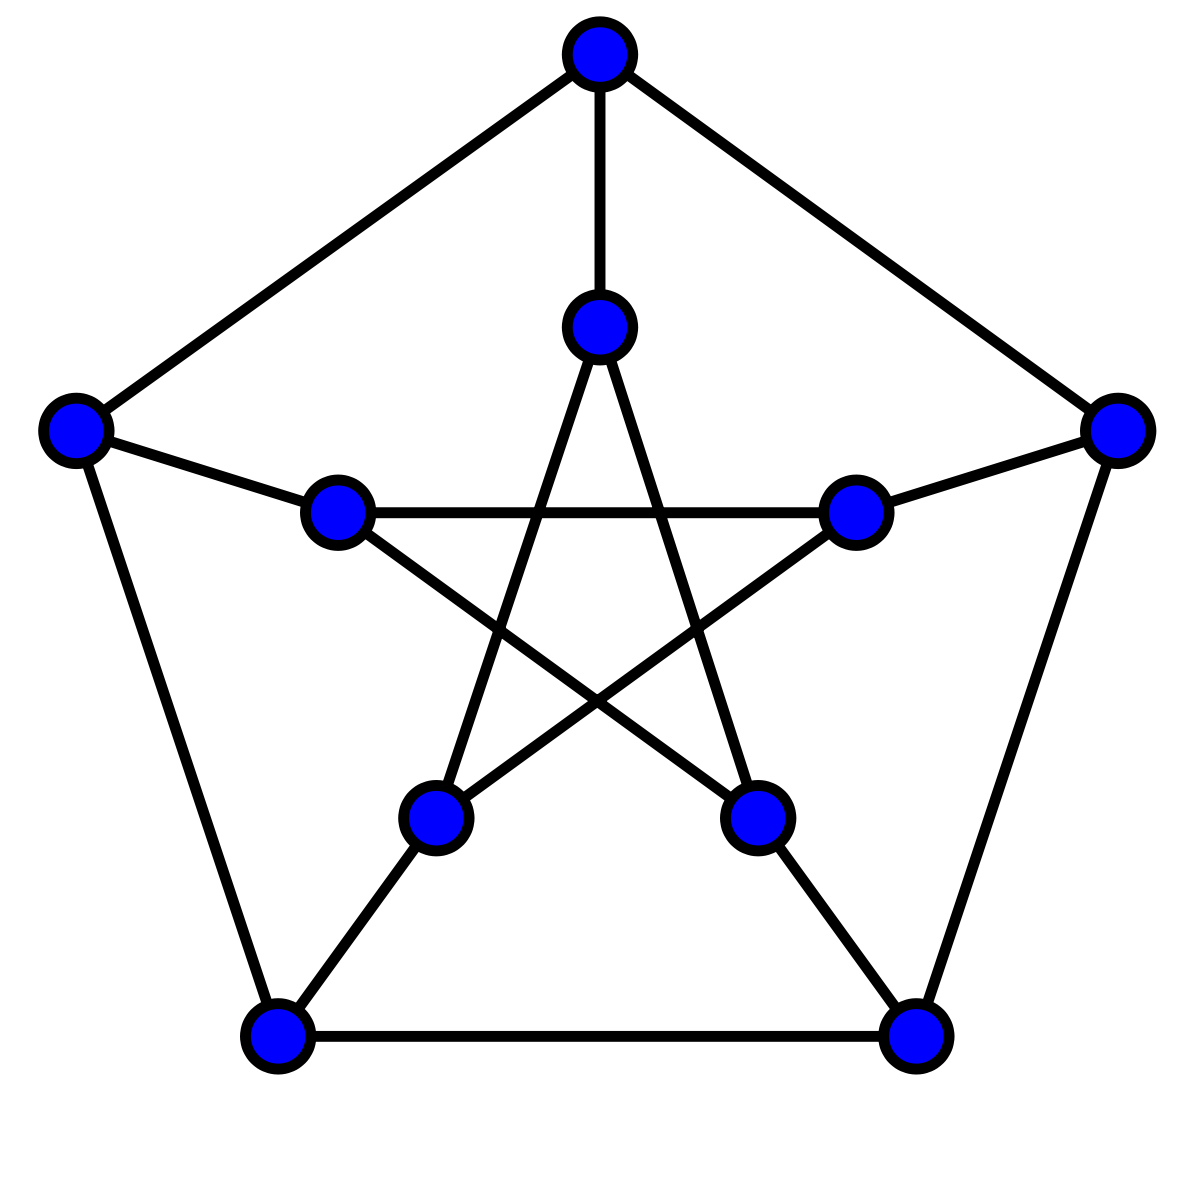
\includegraphics[width=0.9in]{petersen.png} \]
Find a subgraph of the Petersen graph that's a subdivision of $K_{3,3}$. Conclude that the Petersen graph is not planar. Can you find a subgraph of the Petersen graph that's a subdivision of $K_5$?
\item We showed that for a planar graph $G$, $\#E(G) \leq 3\#V(G)-6$. We say $G$ is \emph{maximal planar} if this inequality is an equality. What do maximal planar graphs look like? Draw some.
\end{enumerate}

\end{document}
